\documentclass[tikz,border=10pt]{standalone}
\usetikzlibrary{calc, angles, quotes}

\begin{document}
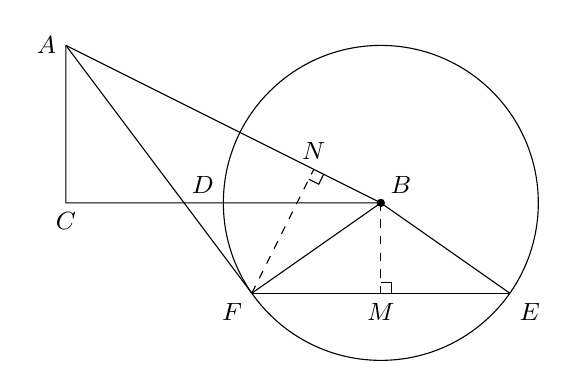
\begin{tikzpicture}[>=stealth, font=\small]

    % 1. 定义基本坐标参数 (基于图像比例估算)
    \coordinate (C) at (0,0);
    \coordinate (A) at (0,2);
    \coordinate (B) at (4,0);
    
    % 2. 绘制圆 B，半径设为 2
    \def\r{2}
    \draw (B) circle (\r);
    \fill (B) circle (1.5pt); % 画出圆心点 B
    
    % 3. 确定圆上的特定交点
    % D 是圆与 BC 的交点
    \coordinate (D) at ($(B) + (-\r, 0)$);
    
    % E, F 位于圆上，且 FE 是水平线。根据原图比例，设其 y 坐标在下方
    \coordinate (F) at ($(B) + ({180+35}:\r)$); % 约 215 度位置
    \coordinate (E) at ($(B) + ({-35}:\r)$);      % 约 -35 度位置


    \coordinate (N) at ($(A)!(F)!(B)$);
    \draw [dashed] (F) -- (N);  % 绘制垂线
    \pic[draw, angle radius=4pt, text=black] {right angle = F--N--B};

    \coordinate (M) at ($(F)!(B)!(E)$);
    \draw [dashed] (B) -- (M);  % 绘制垂线
    \pic[draw, angle radius=4pt, text=black] {right angle = B--M--E};
    % 4. 绘制直线和线段
    \draw (A) -- (C) -- (B) -- (A);           % 直角三角形 ABC
    \draw (A) -- (F);                         % 线段 AF
    \draw (F) -- (E);                         % 线段 FE
    \draw (B) -- (F);                         % 半径 BF
    \draw (B) -- (E);                         % 半径 BE
    
    % 5. 标注文本标签
    % 使用 pos 或 偏移量确保标签不与线条重叠
    \node[left]  at (A) {$A$};
    \node[below] at (C) {$C$};
    \node[above right] at (B) {$B$};
    \node[above left]  at (D) {$D$};
    \node[below left]  at (F) {$F$};
    \node[below right] at (E) {$E$};
    \node[below] at (M) {$M$};
    \node[above] at (N) {$N$};

\end{tikzpicture}
\end{document}